%Pakete;
%A4, Report, 12pt
\documentclass[ngerman,a4paper,12pt]{scrreprt}
\usepackage[a4paper, right=20mm, left=20mm,top=30mm, bottom=30mm, marginparsep=5mm, marginparwidth=5mm, headheight=7mm, headsep=15mm,footskip=15mm]{geometry}

%Papierausrichtungen
\usepackage{pdflscape}
\usepackage{lscape}

%pdf include
\usepackage{pdfpages}

%Deutsche Umlaute, Schriftart, Deutsche Bezeichnungen
\usepackage[utf8]{inputenc}
\usepackage[T1]{fontenc}
\usepackage[ngerman]{babel}

%quellcode
\usepackage{listings}

%tabellen
\usepackage{tabularx}

%listen und aufzählungen
\usepackage{paralist}

%farben
\usepackage[svgnames,table,hyperref]{xcolor}

%font
\usepackage{helvet}
\renewcommand{\familydefault}{\sfdefault}

%Abkürzungsverzeichnisse
\usepackage[printonlyused]{acronym}

%Bilder
\usepackage{graphicx} %Bilder
\usepackage{float}	  %"Floating" Objects, Bilder, Tabellen...

%Dokumenteigenschaften
\providecommand{\project}{WebRTC VoIP Applikation}
\providecommand{\documentType}{Projektplan}
\title{\documentType \project}
\author{Tobias Blaser, Beat Gutzwiller}
\providecommand{\teacher}{Luc Bläser}
\providecommand{\room}{1.267}
\providecommand{\versionnumber}{1.0}
\date{\today{}, Rapperswil}


%Kopf- /Fusszeile
\usepackage{fancyhdr}
\usepackage{lastpage}

\pagestyle{fancy}
\fancyhf{} %alle Kopf- und Fußzeilenfelder bereinigen
\fancyhead[L]{Semesterarbeit} %Kopfzeile links
\fancyhead[C]{\project} %Kopfzeile mitte
\fancyhead[R]{Seite \thepage/\pageref{LastPage}} %Kopfzeile rechts
\renewcommand{\headrulewidth}{0.4pt} %obere Trennlinie
\fancyfoot[L]{\jobname} %Fusszeile links
\fancyfoot[C]{Version: \versionnumber} %Fusszeile mitte
\fancyfoot[R]{\today{}} %Fusszeile rechts
\renewcommand{\footrulewidth}{0.4pt} %untere Trennlinie

%Kopf-/ Fusszeile auf chapter page
\fancypagestyle{plain} {
	\fancyhf{} %alle Kopf- und Fußzeilenfelder bereinigen
	\fancyhead[L]{Semesterarbeit} %Kopfzeile links
	\fancyhead[C]{\project} %Kopfzeile mitte
	\fancyhead[R]{Seite \thepage/\pageref{LastPage}} %Kopfzeile rechts
	\renewcommand{\headrulewidth}{0.4pt} %obere Trennlinie
	\fancyfoot[L]{\jobname} %Fusszeile links
	\fancyfoot[C]{Version: \versionnumber} %Fusszeile mitte
	\fancyfoot[R]{\today{}} %Fusszeile rechts
	\renewcommand{\footrulewidth}{0.4pt} %untere Trennlinie
}

\usepackage{changepage}

%links, verlinktes Inhaltsverzeichnis, PDF Inhaltsverzeichnis
\usepackage[bookmarks=true,
bookmarksopen=true,
bookmarksnumbered=true,
breaklinks=true,
colorlinks=true,
linkcolor=black,
anchorcolor=black,
citecolor=black,
filecolor=black,
menucolor=black,
pagecolor=black,
urlcolor=black
]{hyperref} % Paket muss unbedingt als letzes eingebunden werden!

\begin{document}

%Titel und Inhaltsverzeichnis
\thispagestyle{empty}
\begin{titlepage}
	\begin{center}

	\vspace*{40mm}
	
	\begin{figure}[htp]
		\centering
		
\includegraphics[scale=0.60]{../img/icon-js-voip.png}
	\end{figure}		
	\vspace*{20mm}
	
	{\fontsize{40}{48} \selectfont \project \\[10mm]}
	{\fontsize{40}{48} \selectfont \documentType \\[5mm]}	
	\vspace*{20mm}
	Tobias Blaser, Beat Gutzwiller

\end{center}
\end{titlepage}
\clearpage

\chapter*{Änderungsnachweis}
\begin{tabularx}{\textwidth}{|cXlr|} % Versionstabelle, Rahmen links und rechts
		\hline
		\textbf{Version} & \textbf{Änderung} & \textbf{Autor} & \textbf{Datum}\\
		\hline
		1.0 & Dokumentenentwurf & Tobias Blaser & 23.09.13\\
		1.1 & Infrastruktur, Arbeitspakete & Tobias Blaser & 23.09.13\\
		1.1 & Risikomanagement & Beat Gutzwiller & 03.10.13\\
		\hline
\end{tabularx}

% Inhaltsverzeichnis
\tableofcontents

\chapter{Einführung}

\section{Beschreibung}
Dieses Dokument beinhaltet den Projektplan für das Projekt \project sowie dessen Aufteilung in Arbeitspakete und die Festlegung von Meilensteinen.

\section{Gültigkeitsbereich}
Dieses Dokument ist für das gesammte Projekt \project gültig.

\chapter{Projektorganisation}

\section{Projektteam}
\subsection*{Tobias Blaser}
\begin{figure}[H]
	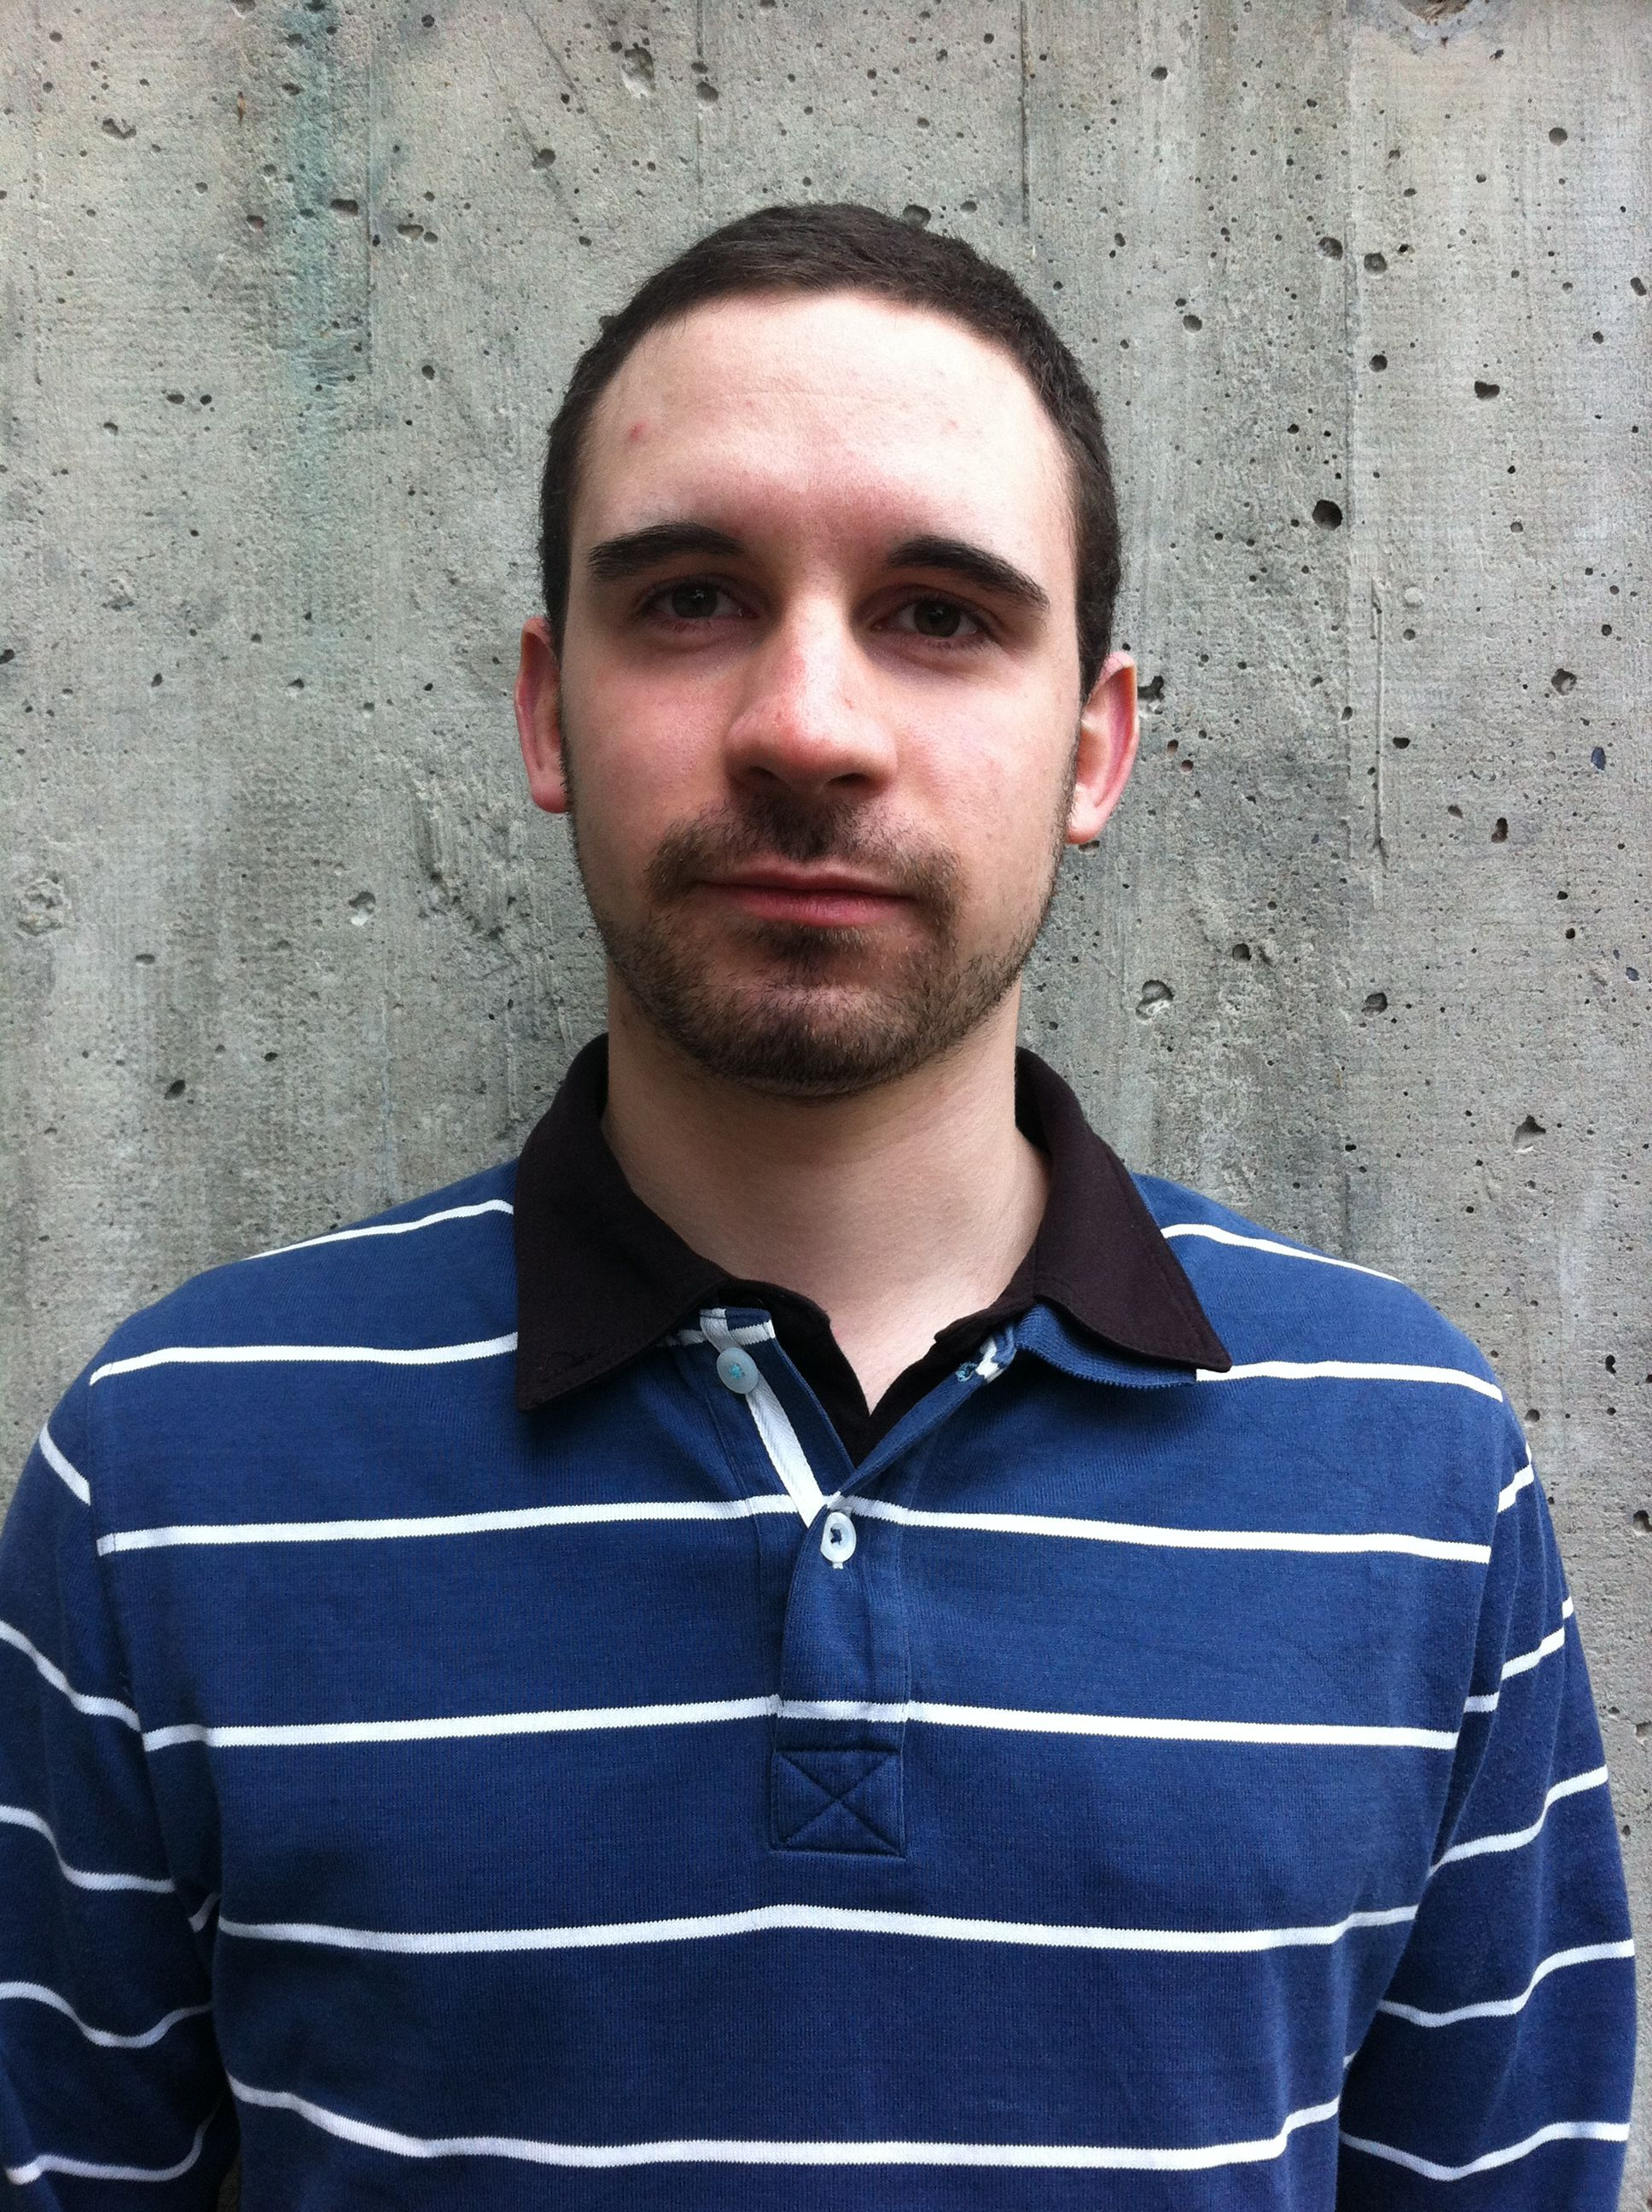
\includegraphics[width=0.3\textwidth]{img/tobias.jpg}
	\centering
	\caption{Tobias Blaser}
	\label{fig:tobias}
\end{figure}

\subsection*{Beat Gutzwiller}
\begin{figure}[H]
	
\includegraphics[width=0.3\textwidth]{img/beat.jpg}
	\centering
	\caption{Beat Gutzwiller}
	\label{fig:beat}
\end{figure}

\section{Externe Schnittstellen}
\teacher\ betreut die Semesterarbeit und begleitet das Team durch regelmässige Meetings.

\chapter{Risikomanagement}
\label{risiken} 
\section{Risiken}

%Die Spalten werden aufgeteilt auf 0.3 resp. 0.7-fache Textbreite
\noindent
\begin{tabular}{|p{0.3\textwidth} | p{0.7\textwidth} |}
	\hline	
	Risiko-ID & 1 \\
	\hline
	Titel & Implementierungshindernis \\
	Beschreibung & Aufgrund einer nicht bedachten Schwierigkeit verzögert sich die
	Entwicklung des Programms. \\
	max. Schaden	& 10h \\
	Eintrittswahrscheinlichkeit & 0.4 \\
	Gewichteter Schaden	& 4h \\
	Vorbeugung	& Sorgfältige Abklärungen im Vorfeld der Implementierung. \\
	Massnahmen	& Zusätzliche Entwicklungszeit, um das Problem zu lösen. \\
	\hline
\end{tabular}
\hspace{0.5cm}
\newline

\noindent
\begin{tabular}{|p{0.3\textwidth} | p{0.7\textwidth} |}
	\hline	
	Risiko-ID & 2 \\
	\hline
	Titel & Verbindungsverlust \\
	Beschreibung & Kurze Unterbrüche in der Verbindung könnten die ganze Session
	beenden. \\
	max. Schaden	& 8h \\
	Eintrittswahrscheinlichkeit & 0.9 \\
	Gewichteter Schaden	& 7.2h \\
	Vorbeugung	& Einarbeitung in SIP Connection Management. \\
	Massnahmen	& Session bei kleinen Unterbrüchen aufrecht erhalten und einen
	schnellen Reconnect einrichten. \\
	\hline
\end{tabular}
\hspace{0.5cm}
\newline
	
	
\noindent
\begin{tabular}{|p{0.3\textwidth} | p{0.7\textwidth} |}
	\hline	
	Risiko-ID & 3 \\
	\hline
	Titel & Browserperformance \\
	Beschreibung & Video und Audio müssen flüssig wiedergegeben werden. \\
	max. Schaden	& 3h \\
	Eintrittswahrscheinlichkeit & 0.1 \\
	Gewichteter Schaden	& 0.3h \\
	Vorbeugung	& Performance-Tests mit Prototypen. \\
	Massnahmen	& Skalierung der Videoqualität, notfalls Priorisierung auf Audio. \\
	\hline
\end{tabular}
\hspace{0.5cm}
\newline
	
	
\noindent
\begin{tabular}{|p{0.3\textwidth} | p{0.7\textwidth} |}
	\hline	
	Risiko-ID & 4 \\
	\hline
	Titel & Langsame Verbindung \\
	Beschreibung & Bei langsamen Verbindungen kann es zu Problemen in der
	Wiedergabe führen. \\
	max. Schaden	& 8h \\
	Eintrittswahrscheinlichkeit & 0.8 \\
	Gewichteter Schaden	& 6.4h \\
	Vorbeugung	& Performance-Tests mit Prototyp und künstlichem Traffic. \\
	Massnahmen	& Skalierung der Videoqualität, notfalls Priorisierung auf Audio. \\
	\hline
\end{tabular}
\hspace{0.5cm}
\newline
	
	
\noindent
\begin{tabular}{|p{0.3\textwidth} | p{0.7\textwidth} |}
	\hline	
	Risiko-ID & 5 \\
	\hline
	Titel & Konferenzschaltung \\
	Beschreibung & Hohe Teilnehmerzahl führt zu hoher Anzahl Verbindungen. \\
	max. Schaden	& 1h \\
	Eintrittswahrscheinlichkeit & 1.0 \\
	Gewichteter Schaden	& 1h \\
	Vorbeugung	& Performance-Tests mit Prototypen. \\
	Massnahmen	& Maximale Anzahl Teilnehmer festlegen. \\
	\hline
\end{tabular}
\hspace{0.5cm}
\newline

	
\noindent
\begin{tabular}{|p{0.3\textwidth} | p{0.7\textwidth} |}
	\hline	
	Risiko-ID & 6 \\
	\hline
	Titel & Kompetenzmangel SIP \\
	Beschreibung & Erfahrung mit SIP mangelt. Unbekannte Probleme möglich. \\
	max. Schaden	& 14h \\
	Eintrittswahrscheinlichkeit & 0.7 \\
	Gewichteter Schaden	& 9.8h \\
	Vorbeugung	& Frühe Einarbeitung in SIP. \\
	Massnahmen	& Zusätzliche Entwicklungszeit. \\
	\hline
\end{tabular}
\hspace{0.5cm}
\newline


\noindent
\begin{tabular}{|p{0.3\textwidth} | p{0.7\textwidth} |}
	\hline	
	Risiko-ID & 7 \\
	\hline
	Titel & NAT \& Firewall Traversal \\
	Beschreibung & NATs und Firewalls lassen sich nicht ohne weiteres durchdringen.
	\\
	max. Schaden	& 20h \\
	Eintrittswahrscheinlichkeit & 0.25 \\
	Gewichteter Schaden	& 5h \\
	Vorbeugung	& Früh Verbindungstests mit NATs und Firewalls durchführen. \\
	Massnahmen	& Zusätzliche Entwicklungszeit investieren zur Unterstützung von
	Proxyservern und Tunneling-Mechanismen. \\
	\hline
\end{tabular}
\hspace{0.5cm}
\newline


\noindent
\begin{tabular}{|p{0.3\textwidth} | p{0.7\textwidth} |}
	\hline	
	Risiko-ID & 8 \\
	\hline
	Titel & Verschlüsselte Verbindung \\
	Beschreibung & Das Verschlüsseln der P2P-Verbindung und des Server-Connects
	gestalten sich schwieriger als gedacht. \\
	max. Schaden	& 16h \\
	Eintrittswahrscheinlichkeit & 0.5 \\
	Gewichteter Schaden	& 8h \\
	Vorbeugung	& Früh Möglichkeiten zur Verschlüsselung und deren
	Implementierungsaufwand analysieren. \\
	Massnahmen	& Zusätzliche Entwicklungszeit investieren zur Umsetzung des
	Verschlüsselungsmechanismus. \\
	\hline
\end{tabular}
\hspace{0.5cm}
\newline


\noindent
\begin{tabular}{|p{0.3\textwidth} | p{0.7\textwidth} |}
	\hline
	Risiko-ID & 9 \\
	\hline
	Titel & Social Risks \\
	Beschreibung & Die Projektmitglieder sind aufgrund anderer Projekte zu stark
	absorbiert und können zu wenig Zeit für das Projekt aufwenden. \\
	max. Schaden & 25h \\
	Eintrittswahrscheinlichkeit & 0.25 \\
	Gewichteter Schaden	& 6h \\
	Vorbeugung	& Externe Projekte in der Iterationsplanung berücksichtigen. \\
	Massnahmen	& Projektmitglieder opfern ihre Freizeit und trinken mehr Red Bull.
	\\
	\hline
\end{tabular}
\hspace{0.5cm}
\newline


\section{Umgang mit Risiken}
Um die Riskien möglichst kalkulierbar zu halten, ist es für dieses Projekt
entscheidend, möglichst früh Evaluationen durchzuführen. Besonders die frühe Einarbeitung in SIP sowie die Bereitstellung eines ersten
Prototypen mit SIP-Verbindung muss gewährleistet werden. Sobald Prototypen
vorhanden sind, müssen erste Performance-Test durchgeführt werden. Weiterhin
sollten die Risiken laufend neu beurteilt werden.

\chapter{Projektplan}
Die einzelnen Arbeitspakete werden mithilfe des Projektverwaltungstools Redmine
organisiert. Für die Betreuer wurde ein eigener Zugang zum Redmine-Projekt eingerichtet.

%\section{Gastzugang Redmine}
%http://152.96.192.44/redmine \\
%Zugang: guest / zurich2Rapperswil \\

	\section{Milestones}
		\subsubsection{Elaboration I2 - MS core prototypes}
			\begin{itemize}
				\item Prototypen der Kernkomponenten, insbesondere der Komponenten mit hohen Risiken
					\begin{itemize}
						\item WebRTC P2P Communication Prototype
						\item SIP Server Connection Prototype
						\item Addressbook Interface Implementation Prototype
						\item Channel Interface Implementation Prototype (XHR Simple Queue Server)
					\end{itemize}
				\item Risikoanalyse
				\item Architekturanalyse
			\end{itemize}
			
		\subsubsection{Construction I2 - MS core functionality}
			\begin{itemize}
				\item Implementation der Kernkomponenten (Prototyp-Komponenten-Elaboration)
					\begin{itemize}
						\item P2P Communication
						\item Channel Reference-Implementation
						\item Addressbook Reference-Implementation
					\end{itemize}
				\item Zwischenstand Projektdokumentation
			\end{itemize}
			
		\subsubsection{Construction I4 - MS final app}
			\begin{itemize}
				\item Implementation der Advanced Komponenten
					\begin{itemize}
						\item Media Scaling
						\item Scallable User Interface
					\end{itemize}
				\item Projektdokumentation
			\end{itemize}
		
		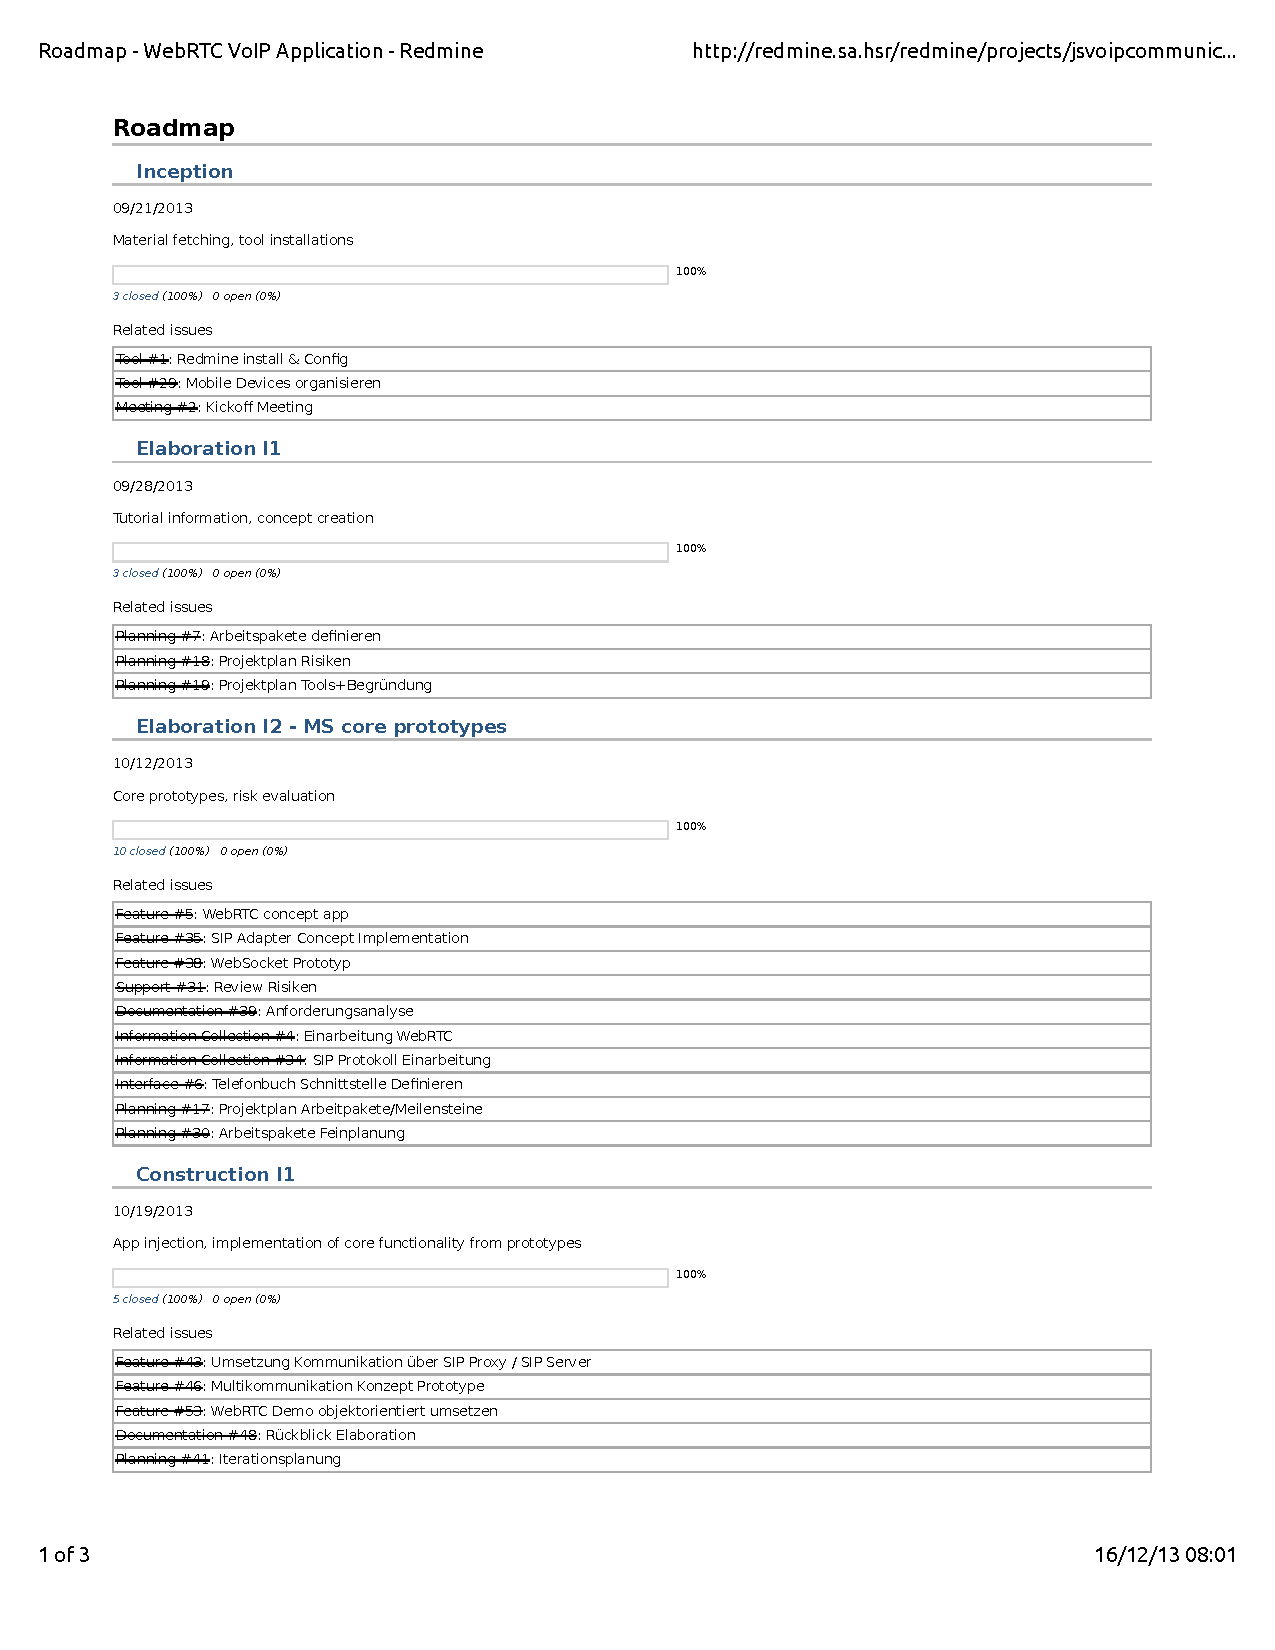
\includepdf[pages=-]{../projektplan/media/roadmap.pdf}
		\begin{landscape}
			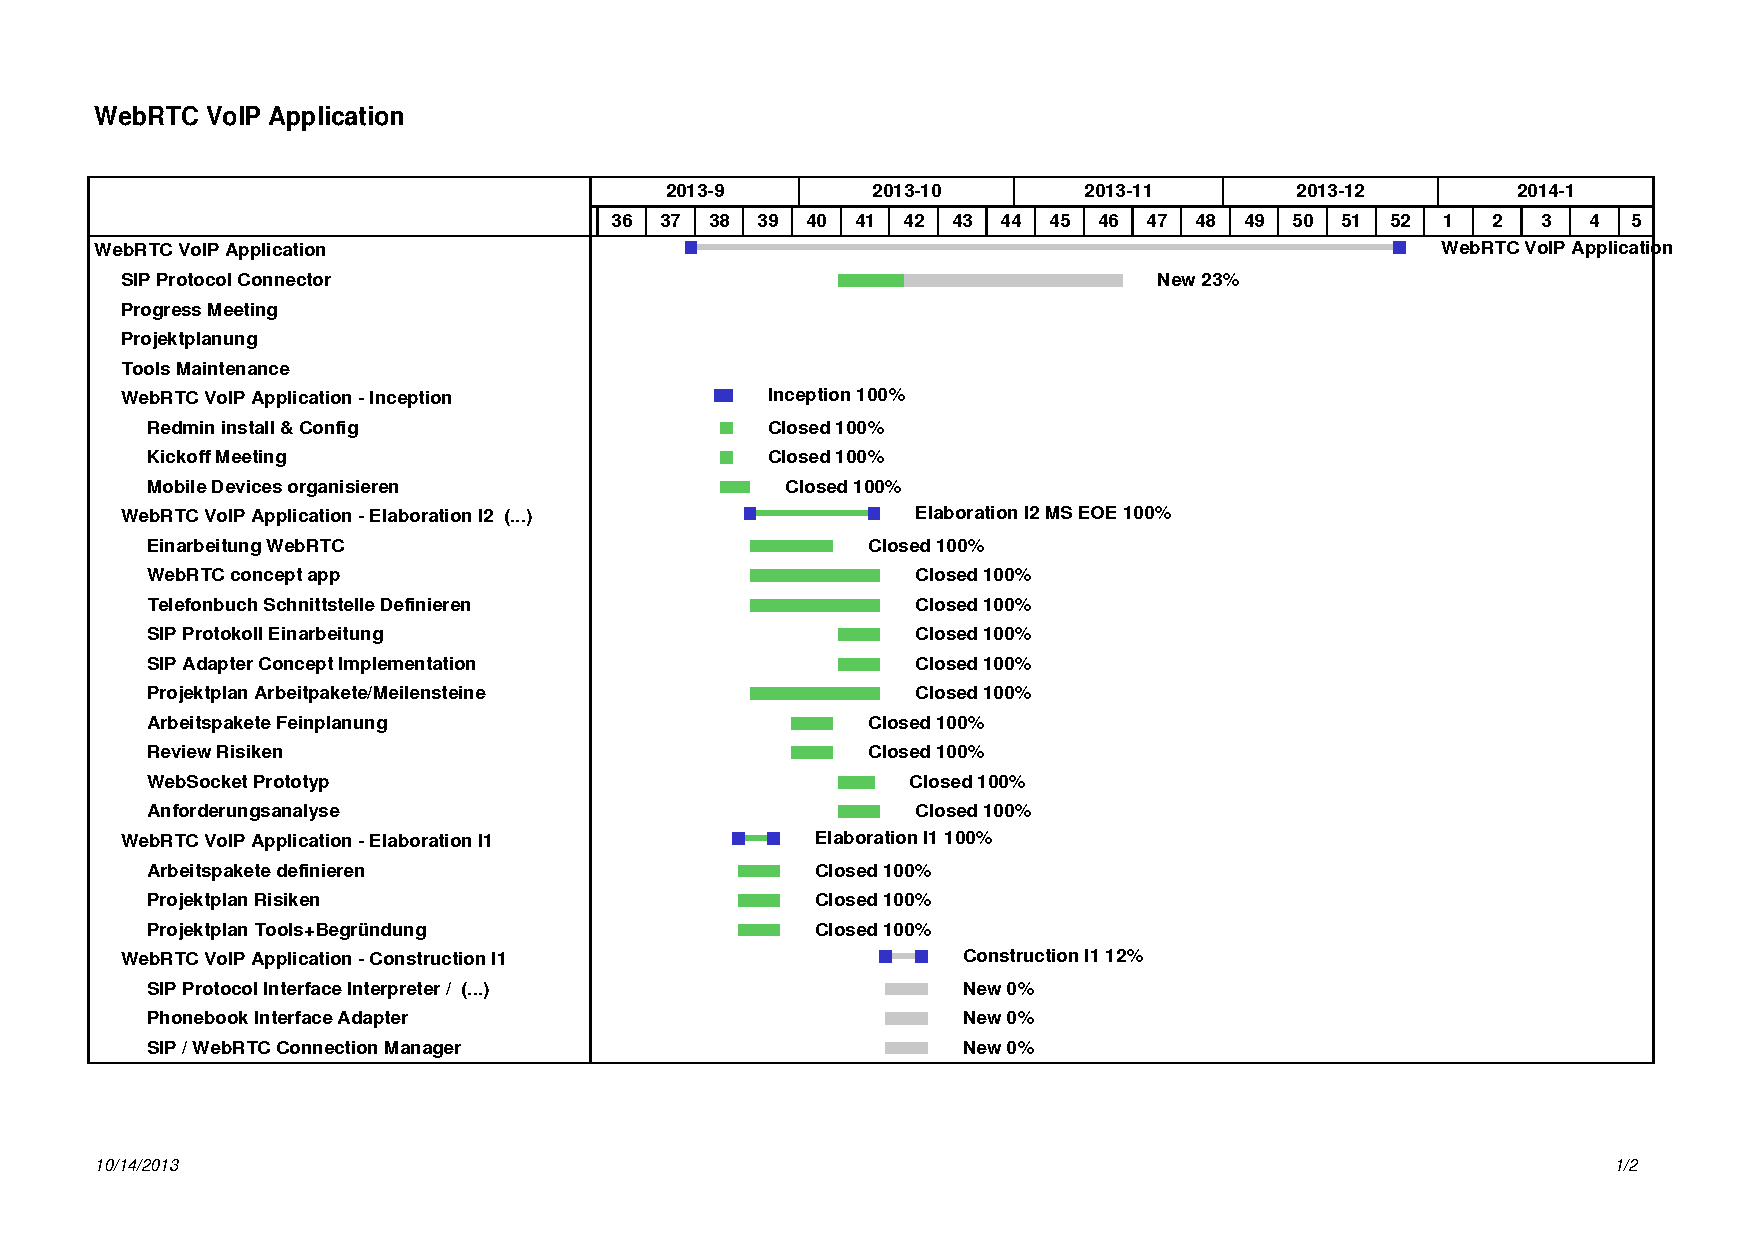
\includepdf[pages=1]{../projektplan/media/jsvoipcommunication-gantt.pdf}
		\end{landscape}
		\begin{landscape}
			\includepdf[pages=2]{../projektplan/media/jsvoipcommunication-gantt.pdf}
		\end{landscape}
		\begin{landscape}
			\includepdf[pages=3]{../projektplan/media/jsvoipcommunication-gantt.pdf}
		\end{landscape}
		
		
	\section{Aufgewendete Zeit}
		\begin{figure}[H]
			\centering
			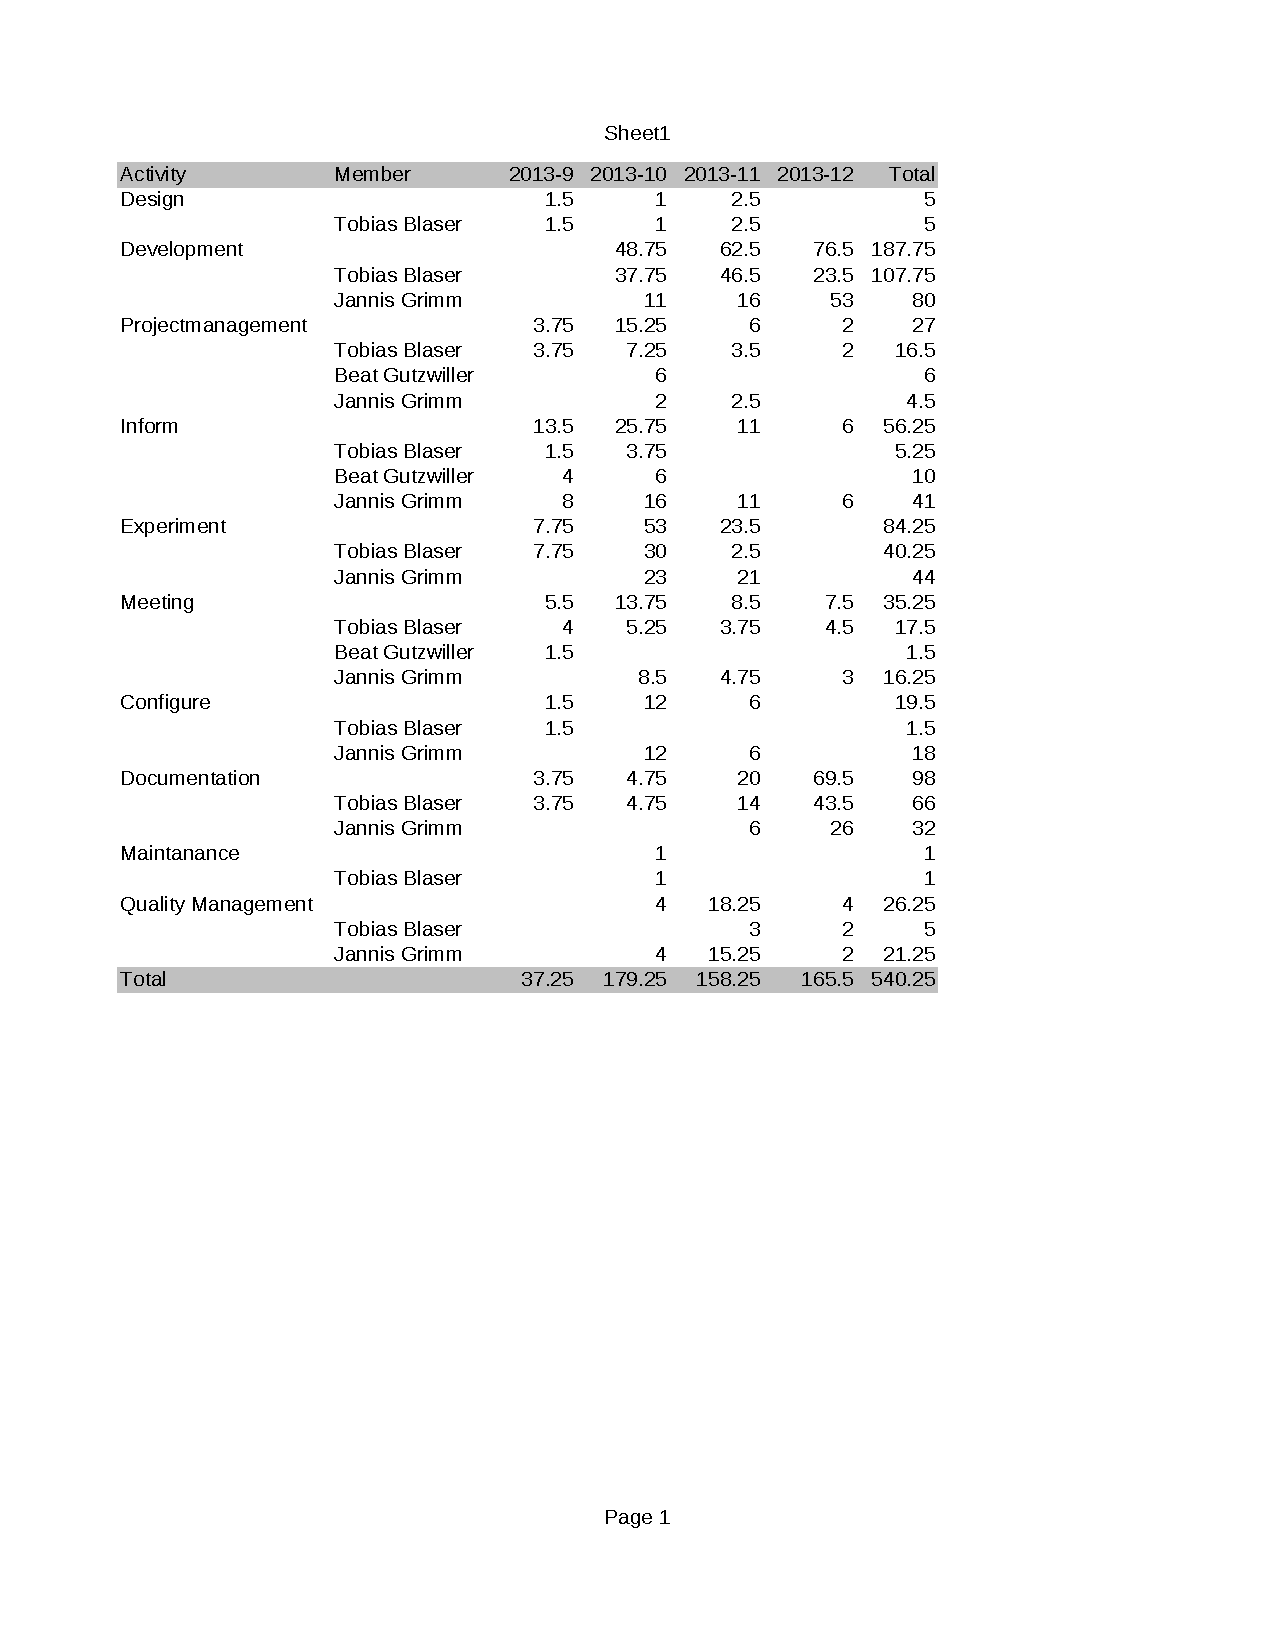
\includegraphics[trim=1.75cm 10cm 5.5cm 2.5cm, clip=true,page=1,width=\textwidth]{../projektplan/media/timelog.pdf}
		\end{figure}
\chapter{Infrastruktur}

\section{Hardware}
\begin{itemize}
	\setlength{\itemsep}{-\parsep}
	\item Persönliche Entwicklungsgeräte für jedes Teammitglied, bevorzugt Laptop (eigene Geräte)
	\item Zugewiesene Arbeitsplätze im Zimmer 1.262
	\item Mobile Devices mit WebRTC fähigem Browser
	\item Virtual Server für Projektmanagement
	\item SIP Service (z.B. sipcall.ch) oder SIP Server
\end{itemize}

\section{Tools}
\subsection{Projektmanagement}
Das Projektmanagementtool Redmine bietet sich aus verschiedenen Gründen an:
\begin{itemize}
	\setlength{\itemsep}{-\parsep}
	\item Redmine ist bekannt vom SE2 Projekt.
	\item Redmine lässt sich auf den Virtual Servern der HSR leicht installieren.
	\item Redmine bietet den benötigten Funktionumfang und ist einfach zu bedienen.
	\item Redmine bietet Git Repository Integration falls dies gewünscht ist.
\end{itemize}


\subsection{Versionsverwaltung}
\subsubsection{Git}
Git ist ein bewährtes Versionsverwaltungstool, bietet den Vorteil von lokalen Repositories, ist sehr schlank und bringt eine gute Merge-Automatik mit.

\subsubsection{GitHub}
Mit GitHub besitzen die Studenten durch andere Projekte bereits Erfahrung. Als Studenten haben sie Zugriff auf kostenlose ``Private-Repositories''. Zudem Bietet GitHub noch zusätzliche Funktionen wie Wiki, RST und MD Viewer sowie Repository Zugriff und Dateibearbeitung über Webinterface.

\subsubsection{Backup}
Ein zusätzliches Backup ist nicht notwendig, da durch die Versionierung mit Git die komplette Versionshistorie bei jedem Teilnehmer vorhanden ist. Somit ist das gesammte Projekt dreifach abgelegt (bei den Entwicklern sowie bei GitHub).


\subsection{Dokumentation}
\subsubsection{Für grosse Dokumentationen und Abgabedokumente: \LaTeX}
\LaTeX ist perfekt geeignet für grosse, gemeinsam zu erarbeitende Dokumente, weil die Source-Dateien über Git versioniert und gemergt werden können und wenig Platz verbrauchen. Zudem besteht ein sehr kleines Risiko auf Dokumentenverlust bzw. Dokumentenfehler durch die Software, weil \LaTeX die Source-Dateien gar nicht verändert im Unterschied zu einer Office Applikation.

\subsubsection{Für Notizen \& Meetingsprotokolle: Restructured Text (rst), txt, Markdown (md)}
Für Notizen und kleine Dokumente reichen RST, TXT oder MD vollständig aus. Sie sind schlank, bieten nur das notwendigste, können versioniert und gemergt werden weil es nur Textfiles sind und werden von "GitHub Document Preview" unterstützt.

\subsubsection{Für Diagramme, Skizzen: Libreoffice Draw (Opendocument)}
Wo es nicht anders geht wird Opendocument eingesetzt. Dabei wird berücksichtigt, dass es über Git nicht inkrementell versioniert und nicht gemergt werden kann.


\subsection{Modelling}
Als Modelling Tool wird Astah gewählt, weil es das beste den Studenten bekannte Tool ist.
Es deckt den geforderten Funktionsumfang grosszügig ab und bietet Image und PDF Export.

\subsection{UI Drafting}
\begin{itemize}
	\setlength{\itemsep}{-\parsep}
	\item Balsamiq Mockup für UI Drafts
	\item ev. Libreoffice Draw für UI Design Finals
\end{itemize}


\subsection{Frameworks}
\subsubsection{Adapter.js}
Adapter.js abstrahiert die verschiedenen Browserschnittstellen von WebRTC und vereinfacht die Entwicklung. Zudem muss bei einer Schnittstellenanpassung browserseitig nur der Adapter aktualisiert werden und nichts an der App geändert werden.

\subsubsection{Ember.js}
Ember.js ist ein bekanntes MVC und Templating Framework, das eine saubere Trennung von Logik und Darstellung ermöglicht. Ember.js bindet darüber hinaus Properties im Template direkt an Objektproperties, wodurch in vielen Fällen eigene Observerimplementierungen überflüssig sind.

\subsubsection{jQuery}
jQuery als eine der besten Javascript Bibliotheken bietet sehr einfache Elementselektoren und viele Funktionen, die das Entwickeln vereinfachen.


\subsection{Testing}
Testing Framework Anforderungen:
\begin{itemize}
	\setlength{\itemsep}{-\parsep}
	\item Testing mit realem Browser, Browsersimulationen unterstützen vermutlich WebRTC noch nicht
	\item Einfach einzubinden
	\item Einfach zu erweitern
	\item Bekannte Benutzung mit Tests und Asserts
	\item Möglichkeit zur Anbindung eines Build Tools
\end{itemize}

\subsubsection{JsUnit}
JsUnit arbeitet mit einem realen Browser, ist einfach handzuhaben und bietet typische Assert-Syntax.


\subsection{Building}
Ein Build Server wie Ant ist nicht nötig für dieses Projekt. JsUnit bietet zwar eine Anbindungsmöglichkeit. Für unsern Anwendungsfall und die nicht sehr komplexe Tool-Umgebung lohnt sich der Aufwand eines Build Servers jedoch nicht.


\subsection{Entwicklungsumgebung}
Jeder Entwickler verwendet seine eigene bevorzugte Entwicklungsumgebung.


\subsection{RunTime Environment}
Als RunTime Environment wird ein WebRTC kompatibler Browser (Firefox, Chrome(ium)) benötigt.




\end{document}
